\section{Design [L]}
Im Designprozess wurden zwei Landingpages in Form von Mockups erstellt (siehe Abbildung \ref{fig:impl:design:mokupsvs}), dafür wurde das Tool Figma benutzt. Die auszuwählende Landingpage soll das weitere Design des GUIs bestimmen.
Zur Auswahl stand ein edlen Design, das in dunklen Farben und eckigen Formaten auftritt.
Das zweite Design ist ein fröhliches Design in bunten und hellen Farben und runden Formen.
Der Auswahlgruppe wurde der Zweck des Prototyps erklärt und die beiden Designs präsentiert.
In der Auswahlrunde erhielt das fröhliche Design das bessere Feedback und wurde ausgewählt.

\begin{figure}[h t]
    \centering
    \includegraphics[scale=0.15]{pics/Design Mockups Gegenüberstellung.png}
    \caption{Landingpage Design Mockups Gegenüberstellung}
    \label{fig:impl:design:mokupsvs}
\end{figure}


\subsection{User Experience [L]}
\setauthor{Litzlbauer Lorenz}
Ein gutes User-Experience-Design ist die Grundlage für eine erfolgreiche Positionierung und Kommunikation mit dem*der Benutzer*in.
UX bezieht sich dabei auf die Interaktion des Benutzers mit der Umwelt, aber auch mit dem angebotenen Service oder Produkt. In diesem Kontext hat Design mehrere Bedeutungen.
Erstens gibt es den Punkt der Gestaltung der Interaktionen, hierzu gehört der Begriff Interface Design (UI Design), er bedeutet visuelle Kommunikation über Zeichen und Symbole.
Zweitens gibt es Design als den Designprozess. Im Designprozess muss erkannt werden, was dem*der Benutzer*in wichtig ist und dieses dem Produkt zugewiesen werden, sodass es auch der*die Benutzer*in erkennen kann \cite{UserExperienceDesign}.

\subsubsection{Anwendungen von UX im Projekt [L]}
Schon beim Projektstart standen die Benutzer*innen im Mittelpunkt. Dazu wurden die in Kapitel User-Stories \ref{ch:user-stories} beschriebenen User-Stories aus Sicht eines Benutzers formuliert, um klar herausarbeiten zu können, welchen effektiven Nutzen unsere Web-Applikation dem*der Nutzer*in bringt.

Die Oberfläche wurde so designt, damit sie leicht verständlich, nützlich und benutzerfreundlich ist. Dafür wurden viele Prototypen (siehe Abbildung \ref{fig:impl:design:prototypesfigma}) in Figma (siehe Kapitel \hyperref[ch::technologies::figma]{Technologien Figma}) gestaltet und durch Umfragen die besten bestimmt und dementsprechende Anpassungen am Design gemacht.

\begin{figure}
    \centering
    \includegraphics[scale=0.5]{pics/ProjektOberflächenDesignPrototypenFigma.png}
    \caption{OberflächenDesign: Prototypen in Figma}
    \label{fig:impl:design:prototypesfigma}
\end{figure}

\subsection{User-Interface-Design [M]}
\setauthor{Fabian Maar}
//TODO

\subsection{Logoentwicklung [M]}
Ein wichtiger Teil der Design-Phase war die Entwicklung eines Logos. Hierbei sollte es darum gehen, ein Wiedererkennungsmerkmal zu schaffen, das sowohl im Gedächtnis bleibt, als auch das Produkt repräsentiert. Um dies zu gewährleisten sollte bei der Logoentwicklung auf folgende Faktoren geachtet werden:

\begin{itemize}
    \item Flexibilität - geeignet für große und kleine Formate
    \item Einzigartig - von der Konkurrenz differenzierbar
    \item innovativer Gestaltungsansatz
    \item Klarheit in der Formensprache
\end{itemize}
\cite{LogoKriterien}

Zur Erstellung des Logos wurde \emph{Adobe Illustrator} verwendet, ein Programm speziell für das Illustrieren von Vektorgrafiken. Für das Logo der Diplomarbeit wurde ein isometrischer Zeichenstil verwendet. Dabei verlaufen alle Fluchtlinien parallel und dadurch erscheint das Design zum einen flach, als auch dreidimensional. Es soll den 3D-Raum symbolisieren, in dem sich ein Podest befindet. Farblich wurde auf eine Abstimmung mit dem Prototypen geachtet, um leichter eine Verbindung mit dem Produkt schaffen zu können.
\cite{IsometricStyle}
\cite{Logo}

\begin{figure} [h]
    \centering
    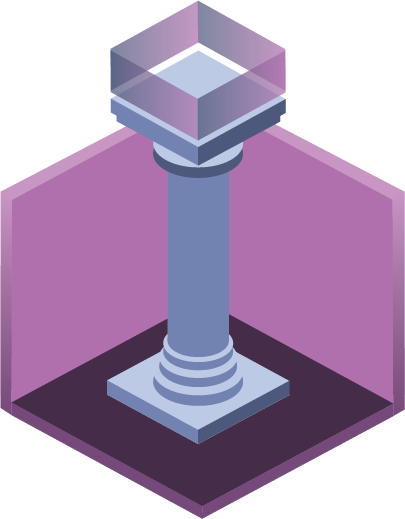
\includegraphics[scale=0.3]{pics/3d-logo.png}
    \caption{Logo der 3D-Portfolio-Galerry}
\end{figure}


%%\subsubsection{UserInterface-Frameworks (UI-Frameworks)}
%%Ein UserInterface-Frameworks ist eine Ansammlung von Web Komponenten wie eine Navigationsleiste die sofort Nutzbar sind.  
%%
%%
%%Die Vorteile von UI-Frameworks sind:
%%\begin{compactitem}
%%    \item vereinfacht und beschleunigt den Entwicklungsprozess;
%%    typische Web-Komponenten sind vordefinierte, der Entwickler muss diese nicht mehr implementieren und erspart sich Zeit.
%%    \item Cross-Browser Unterstützung;
%%    Besonders bei neuen CSS-Feature kann es sein, dass diese noch nicht von allen Browsern unterstützt werden. Ein UI-Framework benutzt in der Regel nur Funktionen, die auch alle Browser anzeigen können.
%%    \item Der Code hat eine bessere Lesbarkeit;
%%    In einem UI-Framework gibt es gewisse Konventionen wie Klassennamen, die befolgt werden müssen. Dadurch wird der Code besser lesbar.
%%\end{compactitem}
%%
%%
%%Die Nachteile von UI-Frameworks sind:
%%\begin{compactitem}
%%    \item Die Ladezeit der Webseite erhöht sich;
%%    Schließlich müssen auch mehr Daten an den Browser geschickt werden.
%%    \item Webseiten, die das selbe UI-Framework verwenden, schauen einander ähnlich aus;
%%    Da die Web-Komponenten gleich implementiert werden.
%%\end{compactitem}
%%\cite{CssFrameworkExplaination} \cite{BestCSSFrameworksin2022}
%%
%%\subsubsection{UI-Frameworks im Projekt}
%%Im Projekt wurde sich für zwei UI-Frameworks, Bootstrap und AngularMaterials, entschieden.
%%
%%
%%\paragraph{Angular Material}
%%Angular Material ist eine UI Framework und wird seit 2014 von Google entwickelt. Das Framework baut auf Angular auf und erweitert es mit eigenen Komponenten, Styleguides, Typographie und vielem mehr. Die Design-Sprache orientiert sich dabei an der Material Design Spezifikation von Google. Ein großer Fokus des Frameworks ist die Responsiveness, Komponenten werden auf verschiedenen Auflösungen gut aussehen.
%%
%%
%%Angular Material hat folgende Features:
%%\begin{compactitem}
%%    \item Erweiterbar; Bei der Installation lassen sich viele Designanpassungen machen, zusätzlich lassen sich Styles mit dem globalen Stylesheet überschreiben. 
%%    \item Hochwertig; Die Komponenten sind erprobt und wurden auf die Performanz und Verlässlichkeit getestet.
%%    \item Reibungslos; Angular Material ist gut mit Angular integriert
%%\end{compactitem}
%%
%%Die Abbildung \ref{fig:impl:angular-material-overview-components} zeigt einen Teil der Komponenten, die Angular Material anbietet. Zu allen diesen Komponenten gibt es eine ausführliche Dokumentation mit Beispiele. 
%%\cite{JavaPointAngularMaterial}
%%\cite{WhatAngularMaterial}
%%
%%\begin{figure}
%%    \centering
%%    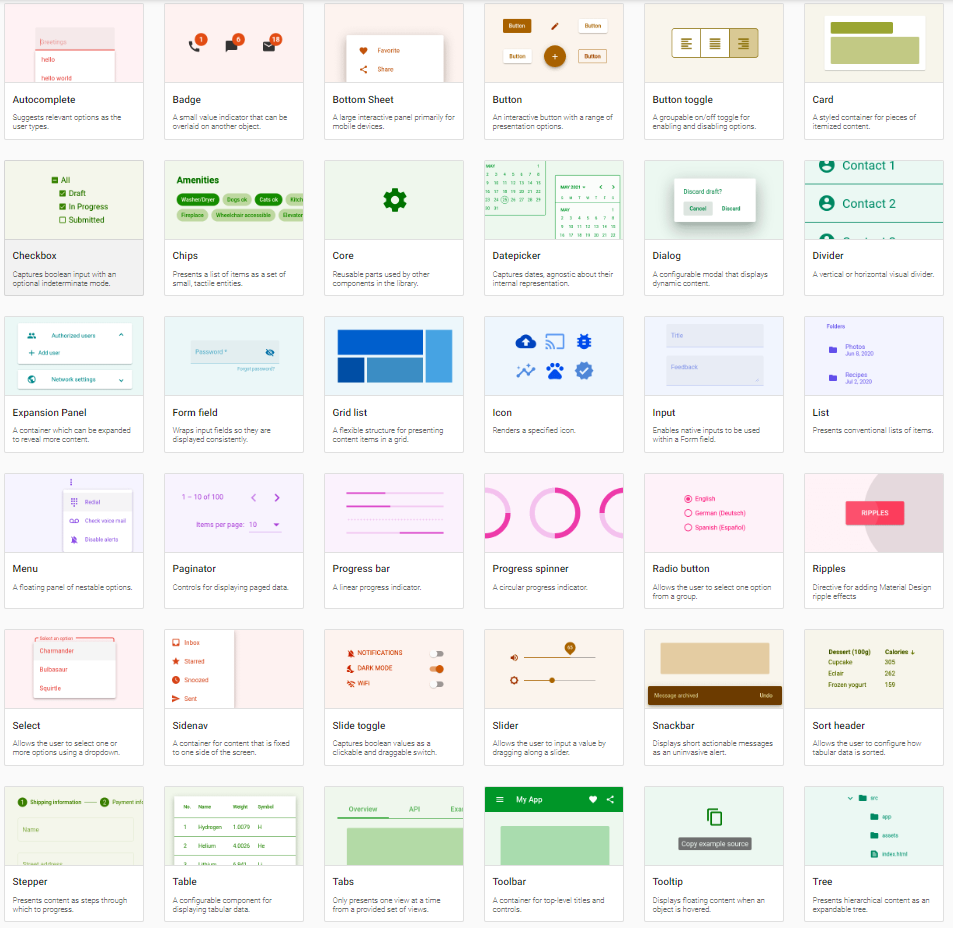
\includegraphics[scale=0.5]{pics/AngularMaterialsComponentsOverview.png}
%%    \caption{Angular Material: Komponente Überblick \cite{AngularComponents}}
%%    \label{fig:impl:angular-material-overview-components}
%%\end{figure}
%%
%%\subparagraph{Material Design Spezifikation}
%%Material Design ist ein Designsystem, welches von Google erstellt wurde, um Teams zu helfen, qualitative hochwertige Digitale-Erfahrungen für Android, iOS, Flutter und das Web zu gestalten.
%%
%%Material Design hat mehrere Prinzipien, die sie ihr Design beeinflussen lassen.
%%
%%Material Design soll die reale Weld abbilden.
%%Text soll durch Typographie, Raster, Abstände, Farben und Bilder soll eine erkennbare Hierarchie entstehen. Komponenten sind interaktive Bauklötze für ein das User Interface. Komponenten haben alle eine Stati-System welches den Status der Komponente fokussiert, selektiert, aktiviert, fehlerhaft, schwebend, gedrückt und ausgeschalten anzeigt. Durch das Theming ist es möglich einzelne Komponenten zu verändern und das Design so anzupassen, dass es zur Corporate Identity der Benutzer*in passt.\cite{MaterialDesign-Introduction}
%%
%%\paragraph{Bootstrap}
%%Bootstrap ist ein kostenloses Open-Source-UI-Framework. Es ist nicht nur eine Ansammlung von CSS sondern auch von JavaScript und HTML code um schöne, interaktive und responsive Webseiten. 
%%
%%Bootstrap hat folgenden Features: 
%%\begin{compactitem}
%%    \item Web-Komponenten, die sofort Anwendbar sind
%%    \item Eine gute Dokumentation
%%    \item Mobile Centered Design
%%    \item Hohe Benutzerfreundlichkeit
%%\end{compactitem}
%%\cite{BestCSSFrameworksin2022}
%%
%%\subsubsection{Scss}
%%SCSS ist kein UI-Framework, sondern vielmehr eine Syntax- und Feature-Erweiterung von CSS, deswegen wurde es schlussendlich auch für dieses Projekt gewählt. SCSS hat viele Vorteile wie zum Beispiel Variablen, Schleifen, Mixins und Imports gegenüber CSS, aber besonders ausschlaggebend war das Prinzip der Verschachtelung.
%%
%%Durch die Verschachtelung kann an redundanten Styles-Selektoren gespart werden, was die Style-Definition besser lesbarer macht. Im den Beispielen (siehe SCSS-Code-Beispiel \ref{lst:imp:design:scss} und natives CSS-Code-Beispiel \ref{lst:imp:design:css}) wird die gleiche Style-Definition von SCSS und CSS ausgedrückt, doch die Schreibweise unterscheidet sich.
%%
%%\cite[Sass Guide]{SassGuide}
%%
%%\begin{lstlisting}[caption=SCSS - Code Beispiel,label=lst:imp:design:scss]
%%nav {
%%    ul {
%%        margin: 0;
%%        padding: 0;
%%        list-style: none;
%%    }
%%    
%%    li { display: inline-block; }
%%    
%%    a {
%%        display: block;
%%        padding: 6px 12px;
%%        text-decoration: none;
%%    }
%%}
%%\end{lstlisting}
%%
%%\begin{lstlisting}[caption=CSS - Code Beispiel,label=lst:imp:design:css]
%%nav ul {
%%    margin: 0;
%%    padding: 0;
%%    list-style: none;
%%    }
%%nav li {
%%    display: inline-block;
%%    }
%%nav a {
%%    display: block;
%%    padding: 6px 12px;
%%    text-decoration: none;
%%}
%%\end{lstlisting}
%%
%%Code Beispiele\ref{lst:imp:design:scss} \ref{lst:imp:design:css} \cite[Sass Guide]{SassGuide}
%%
%%
%%
%%
%%